\documentclass[a4paper]{article}
\usepackage[francais]{babel}
\usepackage[utf8]{inputenc}

\usepackage{graphicx}
\usepackage{fancyhdr}
\usepackage{lastpage}
\usepackage{amsmath}
\usepackage{xspace}
\usepackage{textcomp}

\usepackage{hyperref}

\usepackage[top=30mm, bottom=30mm, left=25mm, right=25mm]{geometry}

\pagestyle{fancy}

\usepackage{helvet}
\usepackage{bbm}

\usepackage{verbatim}
\usepackage{amsmath}
\usepackage[table]{xcolor}
\definecolor{bleugris}{rgb}{.2,.4,.5}

\definecolor{colKeys}{rgb}{0,0,1} 
\definecolor{colIdentifier}{rgb}{0,0,0} 
\definecolor{colComments}{rgb}{0,0.5,1} 
\definecolor{colString}{rgb}{0.6,0.1,0.1} 

\usepackage{listings}

% Permet l'ajout de code par insertion du fichier le contenant
% Les arguments sont :
% $1 : nom du fichier � inclure
% $2 : le type de langage (C++, C, Java ...)
\newcommand{\addCode}[2]{%

  % Configuration de la coloration syntaxique du code
  \definecolor{colKeys}{rgb}{0,0,1}
  \definecolor{colIdentifier}{rgb}{0,0,0}
  \definecolor{colComments}{rgb}{0,0.5,1}
  \definecolor{colString}{rgb}{0.6,0.1,0.1}

  % Configuration des options 
  \lstset{%
    language = #2,%
    identifierstyle=\color{colIdentifier},%
    basicstyle=\ttfamily\scriptsize, %
    keywordstyle=\color{colKeys},%
    stringstyle=\color{colString},%
    commentstyle=\color{colComments},%
    columns = flexible,%
    %tabsize = 8,%
    showspaces = false,%
    numbers = left, numberstyle=\tiny,%
    frame = single,frameround=tttt,%
    breaklines = true, breakautoindent = true,%
    captionpos = b,%
    xrightmargin=10mm, xleftmargin = 15mm, framexleftmargin = 7mm,%
  }%
    \begin{center}
    \lstinputlisting{#1}
    \end{center}
}

\newcommand{\nTitle}[1]{%
	\clearpage
	\vspace*{\fill}		%
	\begin{center}	%
		\part{#1}		%
	\end{center}
	\vspace*{\fill}		%
	\clearpage
}

\newenvironment{nAbstract} 		%
{ 								%
	\newpage 					% 
	\vspace*{\fill}				%
	\begin{center}			 	%
		\begin{abstract}		%
}{								%
		\end{abstract}			%
	\end{center}				%
	\vspace*{\fill}				%
	\newpage					%
}


\newcommand{\nClass}[1]{{\color{bleugris}{\textsl{\textbf{#1}}}}}
\newcommand{\nParameter}[1]{{\color{gray}{\textbf{#1}}}}
\newcommand{\nMethod}[1]{{\color{gray}{\textbf{#1}}}}
\newcommand{\nConstant}[1]{\texttt{\uppercase{#1}}}
\newcommand{\nKeyword}[1]{\textsl{\textbf{#1}}}

\graphicspath{{../SourcesMatlab/}}

% Conversion nombres arabes / romain
\makeatletter
\newcommand{\rmnum}[1]{\romannumeral #1}
\newcommand{\Rmnum}[1]{\expandafter\@slowromancap\romannumeral #1@}
\makeatother

\setlength{\headheight}{14pt}

\fancyhf{}


\makeatletter
\def\clap#1{\hbox to 0pt{\hss #1\hss}}%
\def\ligne#1{%
\hbox to \hsize{%
\vbox{\centering #1}}}%
\def\haut#1#2#3{%
\hbox to \hsize{%
\rlap{\vtop{\raggedright #1}}%
\hss
\clap{\vtop{\centering #2}}%
\hss
\llap{\vtop{\raggedleft #3}}}}%
\def\bas#1#2#3{%
\hbox to \hsize{%
\rlap{\vbox{\raggedright #1}}%
\hss
\clap{\vbox{\centering #2}}%
\hss
\llap{\vbox{\raggedleft #3}}}}%
\def\maketitle{%
\thispagestyle{empty}\vbox to \vsize{%
\vfill
\vspace{1cm}
\begin{flushleft}
\usefont{OT1}{ptm}{m}{n}
\huge \@title
\end{flushleft}
\par
\hrule height 4pt
\par
\begin{flushright}
\usefont{OT1}{phv}{m}{n}
\Large \@author
\par
\end{flushright}
\vspace{1cm}
\vfill
\vfill
\bas{}{\@blurb \vspace{1cm}}{}
}%
\cleardoublepage
}
\def\date#1{\def\@date{#1}}
\def\author#1{\def\@author{#1}}
\def\title#1{\def\@title{#1}}
\def\blurb#1{\def\@blurb{#1}}
\author{}
\title{}
\blurb{}
\makeatother

\usepackage{hyperref}
\hypersetup{
colorlinks=false, % bool: Liens colorés
pdfborder={0 0 0} % Ne pas encadrer les liens
}

\usepackage[final]{pdfpages}
\usepackage{rotating}
\usepackage{eurosym}
\usepackage{lscape}
\usepackage{float}
\usepackage{color}
\usepackage{colortbl}
\usepackage{array}
\usepackage[printonlyused]{acronym}

% définir les commandes ici

% s'il y a beaucoup de commandes et de packages à inclure n'h&ésitez pas
% à mettre tout ça dans un fichier include.tex et l'inclure
% \input{include.tex}

\lhead{PdC2 - Dossier d'Architecture}
\rhead{
\includegraphics [width=1.5cm]{insa-couleur.jpg}}
\rfoot{\thepage\ de \pageref{LastPage}}



\begin{document}
\title{PdC 9 : Environement Technico-pédagogique}
\author{Adrien Brochot, Julien Levesy, Martin Richard, Armand Rossius}

%------------------------------------- Page de titre
\maketitle
%\begin{titlepage}
%~

%\vfill
%\begin{Large}
%Septembre 2011
%\end{Large}
%\vfill
%\end{titlepage}
%----------------------------------------------------

%--------------------------------- Table des matières
\newpage
\tableofcontents
\newpage
%----------------------------------------------- Plan
\section*{Introduction}

L’objectif de ce document est de présenter les différents cas d’utilisation de la plateforme pédagogique que nous proposons de mettre en place.\\

Il doit permettre de résumer de manière claire et synthétique les différents usages possible de la solution que nous proposons par les différents acteurs intervenant dans le cadre de celle-ci.\\

Ces différents cas d’utilisation permettrons de définir de manière claire les besoins fonctionnels de la solution proposée.\\

Nous présenterons dans un premier temps un schéma global d’utilisation de la plateforme pédagogique, puis nous étudierons plus en détails les cas d’utilisation à l’aide de 4 autres diagramme de cas d’utilisation.\\

\newpage
\section{Objectifs fonctionnels}

\newpage
\section{Suite de logiciels utilisés}

\newpage
\section{Type de matériel recommandé}

\newpage
\section{Cout de la Solution}

\paragraph{} Cette partie permet de résumer le budget nécessaire au déploiement de la solution de virtualisation que nous proposons. 

\subsection{Serveurs}


\subsection{Ordonnancement et outils client}

\paragraph{} L'ordonnanceur est, dans notre architecture, couplé avec les outils clients. Nous utilisons pour cela un serveur Dell PowerEdge R210 II permettant une gestion optimale de la répartition de charge sur les différents noeuds d'exécution et l'hébergement des outils client.
\\~
\begin{itemize}
	\item powerEdge R210 II - 2099,00 €
	\item VMware server + 1 an de support : 5859,25€
	\item VMware View Connection + 1 an de support - 1748€
\end{itemize}

\subsection{noeuds d’exécution}

\paragraph{} Ces composant composent le coeur de l'architecture. Nous avons choisi les serveurs Dell PowerEdge R710 équipés des nouveaux processeurs Intel Xeon X5670 dotés de 6 coeurs à 2.93GHz assurant une performance optimale d'exécution de machines virtuelles sur le réseau.
\\~
\begin{itemize}
 	\item Dell PowerEdge R710 + VMware Embedded 4.1 - 8812€ * 6 = 52872€
\end{itemize}

\subsection{stockage}

\paragraph{} La gestion du stockage est ici abordée uniquement à titre indicatif : le plan de déploiement prévoit de réutiliser les serveurs déjà présents dans le département. Cette section donne un aperçu du prix d'un serveur disposant de l'espace nécessaire s'il fallait en racheter.
\\~
\begin{itemize}
 	\item Dell NX3100 - 7181€
\end{itemize}

\subsection{Client}

\paragraph{} Notre politique est de réutiliser au maximum l'éxistant, ainsi les nombreux postes physiques du département seront simplement intégrés à la nouvelle architecture et aucun nouveau poste ne sera à acheter.
\\~
\begin{itemize}
	\item 60 postes clients complets et 60 postes deportes a l'aide de boitiers
	\item KVM et de serveurs Blades , environ 15 postes deportes "Sun".
\end{itemize}

\subsection{Formation}

\paragraph{} Afin que les administrateurs du département soient en mesure de gérer et maintenir l'architecture, il sera nécessaire de leur fournir une formation complète sur les solutions VMware qu'ils seront amenés à utiliser.
\\~
\begin{itemize}
	\item 1840 € + 5 * ( 150€ aller retour paris lyon + 5 * 30€ hotel ) = 3340€
\end{itemize}


\subsection{Total}

\begin{itemize}
	\item 65.918,25€
\end{itemize}
\newpage
\section{Gestion du changement et réutilisation de l'existant}

\subsection{Impact sur l'utilisateur final}

La mise en place d’un système de V.M. implique nécessairement des changements qui impacteront les utilisateurs habituels des machines du département informatique.
L’un des objectifs de ce projet, outre la mise en place du système de V.M., sera de s’atteler à minimiser le plus possible les changements qui affecteront, directement ou non, les utilisateurs. \\\\

Dans un premier temps, nous nous attarderons sur les impacts sur le système une fois celui-ci définitivement mis en place. Lorsque l’utilisateur souhaite se connecter à une session, il lui suffit d’allumer l’une des machines actuellement présentes, s'authentifier via une page d’accueil simple, et de choisir enfin une V.M. existante. Une fois la V.M. démarrée, l’utilisateur ne verra pas de différence par rapport à la situation actuelle.\\
Le fait de s'authentifier et de choisir une V.M. ne constitue pas une difficulté en soi, il n’y a donc pas de procédure mise en place spécifiquement pour aider l’utilisateur sur ce point. Nous verrons cependant par la suite qu’un système de T.P. sera mis en place, permettant à l’utilisateur de découvrir le système de V.M., ce T.P. sera donc l’occasion de faire découvrir ce nouveau système d’authentification à l’utilisateur.\\\\

La principale difficulté réside dans la phase préparatoire précédant l’utilisation de la V.M., à savoir l’installation de V.M. En effet, pour pouvoir disposer de V.M., l’utilisateur devra les créer au préalable.\\
C’est donc sur cela qu’il faudra s’attarder pour assister l’utilisateur dans le changement.
Tout d’abord, il sera prévu un T.P. de 4 heures ayant pour but de présenter le nouveau système aux utilisateurs. Il leur permettra de faire leurs premiers pas avec le système, et notamment de créer leur machine première machine virtuelle.\\
Afin de simplifier au plus la création de machines virtuelles, des images pré-configurées (Windows XP / Seven standards, Linux) seront mises à disposition des utilisateurs, qu’il leur suffira de copier pour pouvoir les utiliser. \\\\

Enfin, afin de laisser à chaque utilisateur le temps de s’adapter au changement, un système de dual-boot sera mis en place pour une période de 2 à 3 mois. Pendant cette période, les utilisateurs auront la possibilité de démarrer une machine soit sur une session standard, soit sur le système d’authentification des machines virtuelles. Les utilisateurs auront donc le temps de s’habituer en douceur au nouveau système, et de récupérer leur données. Après un temps, le système de dual-boot sera abandonné au profit des machines virtuelles uniquement.

\subsection{Plannification du changement}

	Les modification apportées à l’infrastructure du réseau du département seront relativement importantes et devront peu à peu être appliquées à tous les postes clients. Un processus de déploiement doux sera pour cela mis en place afin de faciliter la mise en place de la nouvelle architecture. \\
	Pour commencer, les travaux pourront en grande partie s’effectuer pendant des vacances scolaires ou les grandes vacances d’été où le nombre d’utilisateurs des postes du département sera limité. \\
La première étape consistera à libérer de la place dans les locaux techniques des serveurs afin d’installer les nouveaux ESXi nécessaires à la mise en place de notre infrastructure virtuelle. Pour cela, il faudra désactiver un certain nombre de postes. Une première vague de serveurs de stockage sera alors effacée et, en utilisant la nouvelle infrastructure vmware, les administrateurs pourront créer les premières VM. \\
Le but de cette étape sera de configurer le réseau mis en place, de connecter notre infrastructure de virtualisation au serveur d’authentification LDAP déjà présent afin de créer les comptes utilisateurs sur la plateforme. Durant toutes ces étapes, la majeure partie des équipements du département resteront disponibles. Les utilisateurs auront toujours accès à leurs sessions actuelles.\\
	L’étape suivante sera le début de la migration des postes clients pour qu’ils puissent s’intégrer à la nouvelle infrastructure et commencer à l’exploiter. Pour les postes physiques, il sera possible d’installer un système de dual-boot permettant de faire le pont entre les deux technologies. Il sera alors possible de se connecter aux anciennes sessions jusqu’à la suppression des serveurs de données actuels. Les autres postes seront quant à eux remplacés en dernier sans phase de transition. \\
Une fois les tests de fonctionnement effectués dans la première architecture minimale, il sera possible d’intégrer tous les ESXi et de migrer les données sur les nouvelles sessions de chaque utilisateur. Dans la nouvelle infrastructure, chaque utilisateur dispose d’un espace de stockage fixe qu’il est libre d’aménager à sa convenance. Lors de la création des comptes utilisateurs, les administrateurs leur fourniront une VM Windows et une Linux leur permettant de migrer leurs données de leurs deux session et de disposer des mêmes systèmes. \\

\subsection{Formation des administrateurs}

Afin de permettre aux administrateurs du système informatique du département d’assurer une installation et une administration correcte et efficace du nouveau système de machines virtuelles, des formations par des experts de l’équipe VMware seront ogranisées. Ces formations se dérouleront à Paris ; la formation durera 5 jours, et sera financé par le département ; le trajet et le séjour seront entièrement remboursés, à hauteur d’un plafond qu’il convient de fixer en fonction des tarifs en vigueur (le budget actuel prévoit 150€ pour un aller-retour Lyon / Paris et 30€ par nuit d’hôtel).

\subsection{Réutilisation de l'existant}

Dans un soucis de minimiser les coûts, et de simplifier au plus la mise en place du système de machines virtuelles au sein du département informatique, une politique de réutilisation de l'existant a été mise en place.\\
Les principaux points mis en avant par cette politique sont les suivants :
\begin{itemize}
\item[Les serveurs de données] : Les serveurs de données disposent actuellement de suffisamment d'espace pour stocker les données personnelles des étudiants. C'est pourquoi il a été décidé de les conserver et de les utiliser pour stocker les images des machines virtuelles mises à disposition des étudiants. La réutilisation de ces serveurs permet d'éviter l'acquisition couteuse de nouveaux serveurs destinés au stockage de données.
\item [Les postes clients] : Le département informatique dispose déjà de nombreuses machines, et il serait totalement impensable de se débarasser de la totalité du parc matériel mis à disposition au sein du département. Il a donc été décidé de conserver les machines déjà présentes afin d'éviter tout coût inutile. Ces machines seront à termes remplacées par de simple KVM reliées par le biais de KVM switchs aux machines virtuelles. Cependant, cette migration progressive vers un parc de KVM ne fera qu'en parallèle du remplacement normal des machines actuelles, dues à leur obsolescence. Cela ne génère donc pas de coût supplémentaires concernant le parc de machines clientes ; cela permettra même de réduire les coûts de remplacement du parc de machines actuels puisqu'une KVM coute (évidemment) bien moins cher qu'une machine standard.

\end{itemize}


\newpage
\section{Scénario de création d'un T.P. avec captures d'écrans}

Afin de commencer la préparation d’un TP dans la nouvelle architecture virtuelle, l’enseignant souhaitant proposer un TP à ses étudiants doit se connecter au serveur principal à l’aide de vsphère client.
Les comptes des enseignants disposeront de droits afin de pouvoir créer des template de VM permettant de générer les machines de TP. (Lors de la réalisation d’un TP, les étudiants se loggerons selon la même procédure, leurs comptes leur permettant uniquement d’administrer leurs machines personnelles et récupérer les machines virtuelles mises à disposition par les enseignants\\

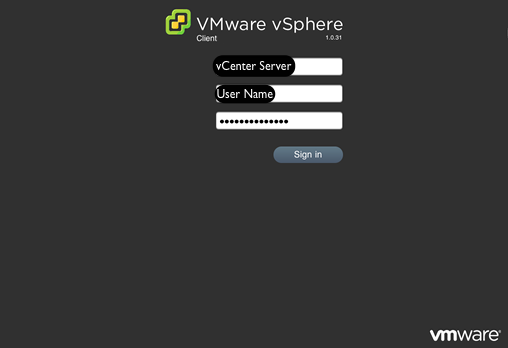
\includegraphics{Login.png}\\


Une fois connecté sur le vSphere Client, l’enseignant a accès à l’ensemble des puissants outils d’administrations fournis par VMware.
L’enseignant, afin de préparer son T.P., devra tout d’abord créer une machine virtuelle (ou en copier une existante, ce qui sera détaillé plus tard) correspondant aux besoins de son T.P. Il pourra par exemple créer une machine virtuelle dont l’objectif sera de permettre aux étudiants de réaliser des tâches d’administration réseau. Il lui suffit pour cela de cliquer sur File -> New -> Virtual Machine. L’assistant de création de machine virtuelle est alors lancé, et il suffit de suivre les indications pour créer la machine virtuelle.\\

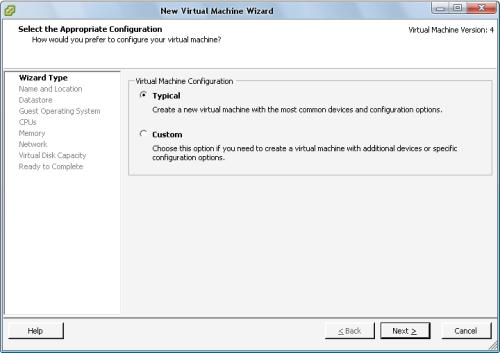
\includegraphics[scale=0.73]{newVM.png}\\

L’enseignant doit maintenant créer un template de machine virtuelle (clic droit sur la machine cible -> clone to Template). Ce template sera une machine virtuelle que les étudiants auront la possibilité de copier (cloner) afin de pouvoir travailler sur leur propre machine virtuelle. Afin que les étudiants puissent avoir accès à ce template, l’enseignant devra le place lors de se création dans un dossier auquel les étudiants ont des droits en lecture.\\

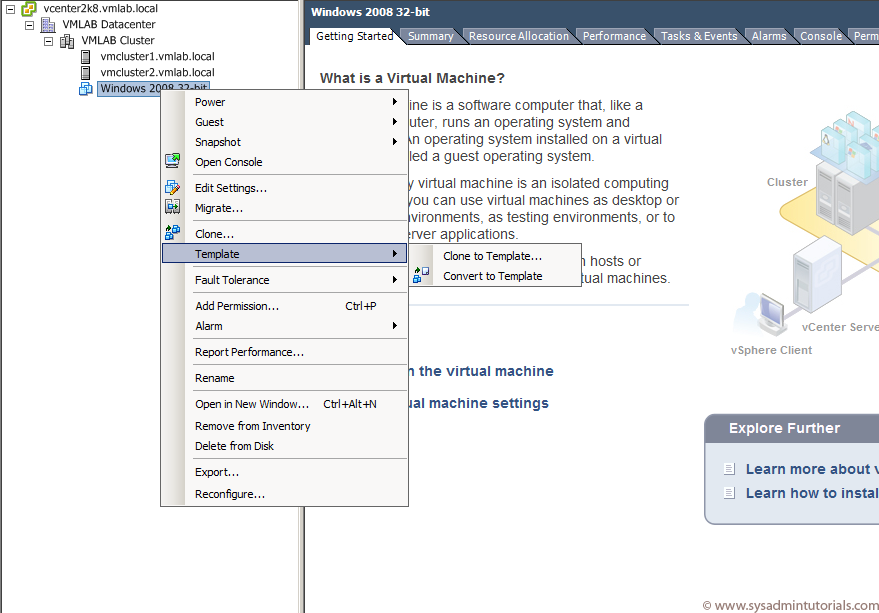
\includegraphics[scale=0.3]{template1.png}\\

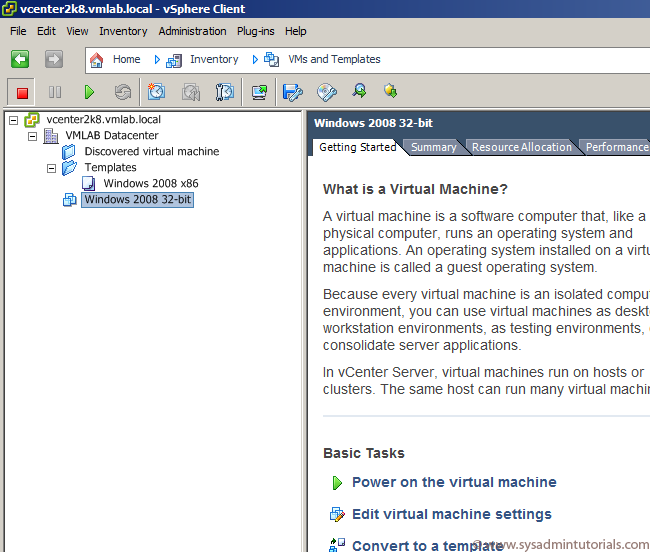
\includegraphics[scale=0.3]{template2.png}\\

Une fois la machine virtuelle créée par l’enseignant, lors de la première séance de TP, les étudiants devront, par groupe, cloner la VM afin d’en avoir chacun une à disposition. Le TP peut alors se dérouler comme un TP normal. L’enseignant pourra cependant facilement monitorer les travaux des étudiants en temps réel et les assister en ouvrant une deuxième console sur les VMs de travail.\\

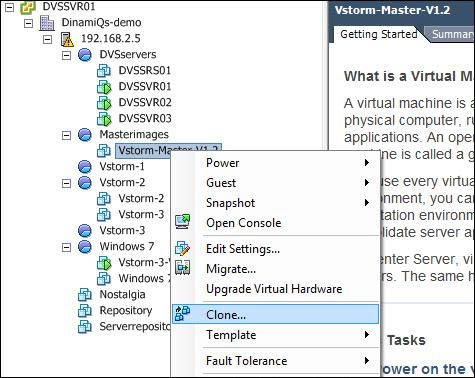
\includegraphics[scale=0.4]{clone.jpg}\\

Une fois le T.P. réalisé par l’étudiant, celui-ci devra prendre un snapshot de sa machine virtuelle. L’enseignant ayant accès à la machine virtuelle que l’étudiant a cloné, il lui suffira de restaurer l’état de la machine pour contrôler le travail de l’étudiant. Il aura évidemment la possibilité de vérifier l’heure à laquelle le snapshot a été pris, ou bien encore de retirer les droits d’écriture sur le dossier dans lequel l’étudiant doit créer sa V.M afin d’éviter toute fraude.\\

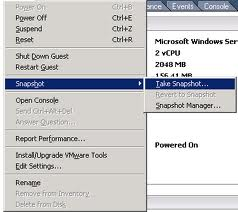
\includegraphics{snapshot.jpg}\\

Comme il est possible de la constater, l'utilisation de la plateforme pédagogique est extrèmement simple, et très intuitive. Les nombreuses fonctionnalités disponnibles (dont il est impossible de fournir une liste exhaustive dans ce document) devraient permettre aux utilisateurs de la plateforme pédagogique d'obtenir entière satisfaction de celle-ci.

\end{document}

